%-*- coding: UTF-8 -*-
\documentclass[hpyerref,UTF8,a4paper,titlepage,12pt,oneside]{ctexbook}
\usepackage{hyperref}
\usepackage{geometry}
\usepackage{xeCJK, fontspec, xunicode, xltxtra,ulem}
\usepackage{amsthm}
\usepackage{amsmath}
\usepackage{amssymb}
\usepackage{mathrsfs}
\usepackage{mathtools}
\usepackage{commath}
\usepackage{listings}
\usepackage{float}
\usepackage{xcolor}
\usepackage{mdframed}

% \graphicspath{{../images/}}
\geometry{a4paper,bottom=2cm}

\title{李群李代数及bundle adjustment}
\author{陈国庆}
\date{\today}

\bibliography{plain}

% 定理结构
\theoremstyle{definition}
\newtheorem{definition}{定义}[section]
\newtheorem{theorem}{定理}[section]
\newtheorem{corollary}{推论}[theorem]
\newtheorem{lemma}[theorem]{Lemma}
\renewcommand\qedsymbol{$\blacksquare$}

\begin{document}

\maketitle
\tableofcontents

\section{群}

$G$是一个集合,在$G$上定义\textit{群乘法}($\cdot$),$G$及对应的乘法($\cdot$)满足下面4个条件,则称$(G,\cdot)$为群,

\begin{itemize}
	\item \textbf{封闭性},$g\cdot h \in G,\quad \forall g,h \in G$
	\item \textbf{结合律},$g\cdot(h\cdot k) = (g\cdot h)\cdot k$
	\item \textbf{单位元},$\exists e\in G$,$g\cdot e = e\cdot g = g,\quad \forall g \in G$
	\item \textbf{逆元},$\exists g^{-1} \in G$,使得$g\cdot g^{-1} = e, g^{-1}\cdot g = e,\quad \forall g \in G$
\end{itemize}

群定义不要求满足\textit{交换律},群乘法($\cdot$)通常可以省略,$g\cdot h$记为$gh$,$(G,\cdot)$记为 $G$。\\

把$\mathbb{R}$作为一个集合,群乘法定义为实数加法,则$(\mathbb{R},+)$构成一个群;若把群乘法定义为实数乘法,则无法构成群,因为0没有逆元。\\

这里一定要清楚,无论群元是什么类型,群上只定义了一种运算,就是群乘法,对群$(\mathbb{R},+)$而言,除了加法其他实数运算都跟群没有关系。

\subsubsection*{\textbf{一般线性群}$GL(n)$}
$$
	GL(n) = \left\lbrace A \in M_{n\times n}|\det(A) \ne 0\right\rbrace
$$
是定义在$\mathbb{R}$上的,$n$阶可逆矩阵的集合,群乘法定义为矩阵乘法。

\subsubsection*{\textbf{特殊正交群}$SO(n)$}

$$
	SO(n) = \left\lbrace R \in M_{n\times n}|RR^T = 1,\det(R) =1\right\rbrace
$$
是单位旋转矩阵的集合,$SO(2),SO(3)$对应二维及三维旋转矩阵。

\subsubsection*{\textbf{特殊欧式群}$SE(3)$}
	通常通过齐次坐标,将旋转、平移用一个$4\times 4$矩阵来表示,
	$$
		T = \begin{bmatrix}
		R_{3\times 3} &\quad \mathbf{v}_{3\times 1}\\
		\mathbf{0}_{1\times 3} &\quad 1
		\end{bmatrix}
	$$
	其中$R \in SO(3)$是一个旋转矩阵,$\mathbf{v}$是一个平移向量,很明显$T$是可逆的,所以$T \in GL(4)$,因为其形式特殊又称为$SE(3)$或,特殊欧式群。\\

	群乘法依然定义为矩阵乘法,可以验证该定义封闭。

\subsubsection*{群同态}
	群同态是两个群之间保群乘法的映射,具体来说,映射$\pi$
	$$
		\phi: G \mapsto G^\prime
	$$
	满足
	$$
		\phi(gh) = \phi(g)\phi(h)
	$$

	比如,$G$为$n\times n$矩阵集合,群乘法定义为矩阵相乘;$G^\prime = \mathbb{R}$,$\phi$为取行列式运算,根据线性代数可知,
	$$
		\det(AB) = \det(A)\det(B)
	$$

	所以$\det$是$G$与$\mathbb{R}$之间的同态映射。\\

	同态映射构造了两个群乘法之间的对应关系,可以借助$G$中的操作构造$G^\prime$中的操作。\\

	比如说,向量空间$V$与某群$G^\prime$之间存在同态映射$\phi$,如何在$G^\prime$上定义微小增量呢?\\

	我们知道在向量空间$V$上定义增量为$x + dx$,可借助同态映射$\phi$,
	$$
		\phi(x+dx) = \phi(x)\phi(dx)
	$$

	来完成$G^\prime$上增量定义。\\

	实际上,李群导数正是借助李代数与李群之间的同态映射构造增量求解导数,这个映射为指数映射。

\subsubsection*{群同构}
	如果同态映射是一一的且是满的,相当于存在逆映射,则称两个群同构。\\

	比如$SO(2)$,为2D平面旋转矩阵群,群员可表示为,
	$$
		A(\theta) = \begin{bmatrix}
			\cos\theta &\quad -\sin\theta\\
			\sin\theta &\quad \cos\theta
		\end{bmatrix}
	$$

	定义映射,
	$$
		f: SO(2) \mapsto \mathbb{R}
	$$

	$$
		f(A(\theta)) = \theta
	$$

	根据旋转矩阵的性质容易验证,$f$是同态映射,并且旋转矩阵与$\theta$是一一对应的,所以$SO(2)$与$\mathbb{R}$同构。\\

	从结构上来讲,两个群同构则认为二者“完全相同”,比如旋转角$\theta$与旋转矩阵是一回事。\\

	对固定的$g\in G$,定义映射,
	$$
		\phi(h) = ghg^{-1}
	$$

	容易验证这个映射是$G\mapsto G$的同构,称为\textbf{伴随同构}。
\section{流形}
	\textbf{微分流形}$M$是一个集合,$n$维流形是指该集合局部同胚与$\mathbb{R}^n$上的开集,所谓同胚是可逆的光滑映射;\\

	\textbf{微分流形}是在拓扑流形基础上施加了进一步约束,称为\textbf{微分结构},具体来说,\\

	$p,q \in M$,$p$的邻域为$U$,$q$的邻域为$V$,则\\

	根据定义,存在同胚映射$\phi: U\mapsto \mathbb{R}^n$,$\psi: U\mapsto \mathbb{R}^n$,对$U\cap V$上的点,需符合映射,
	$$
		\phi\circ\psi^{-1}: \mathbb{R}^n \mapsto \mathbb{R}^n
	$$
	是光滑映射。\\

	根据定义,流形是有维数的,很明显$\mathbb{R}^n$均为$n$维流形,流形定义是脱离坐标系的。

\subsubsection*{微分同胚}

两个微分流形$M,M^\prime$,如果存在可逆的光滑映射$f: M\mapsto M^\prime$,且其逆映射$f^{-1}$也光滑,则称$M,M^\prime$ \textbf{微分同胚}。\\

两个群同构则认为其“完全一样”,相似的两个流形微分同胚则认为“完全一样”。

\subsubsection*{二维球面$S^2$}
三维空间中的球面是一个2维流形,用$S^2$表示,为什么是2维流形呢?在半径确定的情况下,用两个角度即可表示球面上任意点,所以是2维。\\

若要通过坐标系描述$S^2$,则需在三维空间中完成,因此,准确说,$S^2$是嵌入三维空间的二维流形。

\subsubsection*{矢量}
	在$R^n$中“矢量”的意义是明确的,是有大小、有方向的“箭头”,并且与箭头的起始位置无关。\\

	一般流形上没有定义“大小”、“方向”这些概念,那矢量的本质是什么呢?\\

	考虑某个向量$\mathbf{v} = (v_1,v_2,v_3)$,函数$f(x,y,z)$沿$\mathbf{v}$的方向导数为,
	$$
		D_\mathbf{v}(f) \equiv\nabla_f \cdot \mathbf{v}
	$$

	由此看出矢量$\mathbf{v}$可看作$\mathscr{F} \mapsto \mathbb{R} $的映射,$\mathscr{F}$是$\mathbb{R}^3\mapsto \mathbb{R}$的函数集合。\\

	容易验证,$D_\mathbf{v}$是线性映射,

	$$
		D_\mathbf{v}(\alpha f+ \beta g) = \alpha D_\mathbf{v}(f) + \beta D_\mathbf{v}(g)
	$$

	且满足莱布尼兹律,
	$$
		D_\mathbf{v}(fg) = fD_\mathbf{v}(g) + gD_\mathbf{v}(f)
	$$

	由此可见,矢量本质是一个线性映射,推广到一般流形,定义为:\\

	\textbf{流形$M$上的矢量$v$是$\mathscr{F}_M \mapsto \mathbb{R} $的,满足莱布尼兹律的线性映射。}\\

	即,
	\begin{equation} \label{v_linear}
		v(\alpha f+ \beta g) = \alpha v(f) + \beta v(g),\forall f,g \in \mathscr{F}_M,\forall \alpha,\beta \in \mathbb{R}
	\end{equation}

	及
	\begin{equation} \label{v_leb}
		v(fg) = fv(g) + gv(f),\forall f,g \in \mathscr{F}_M
	\end{equation}

	大多数几何书上对矢量的定义就到此为止了,很难从这个定义“想象”出流形上的矢量到底长什么样子,因为这个定义没有揭示方向导数更本质意义。\\

	\begin{figure}[H]
		\begin{center}
			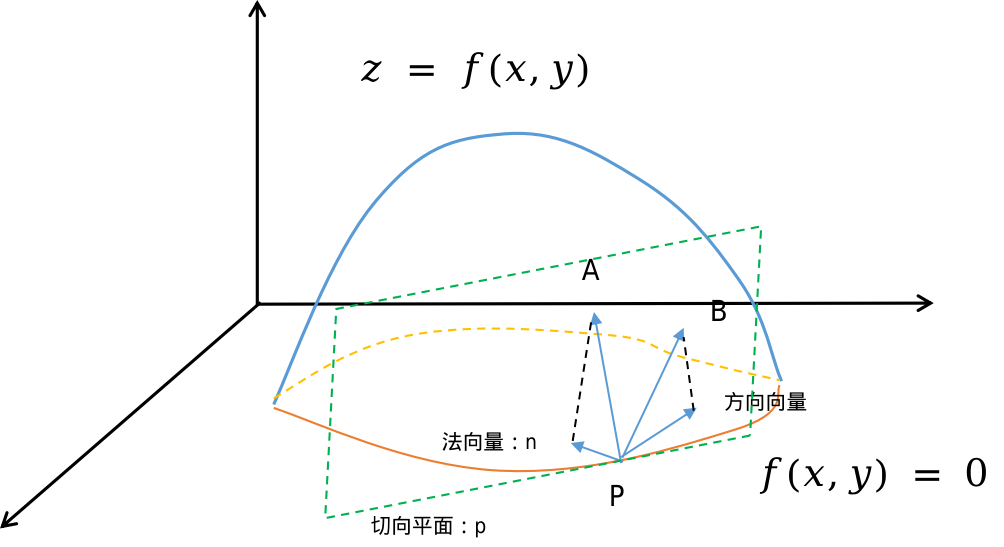
\includegraphics[width=0.8\textwidth]{images/direct_vector.png}
		\end{center}
		\caption{方向向量、方向导数、法向量、切平面}
	\end{figure}	

	如图所示,$z=f(x,y)$的曲面代表一座山,曲面在$P$的切面是绿色平面$p$,$P$点对应的等高面是$f(x,y) = 0$\\

	可以沿着$PA,PB$两个方向(称为\textbf{方向向量})走,因为必须顺着山坡走,所以$PA,PB$都相切于曲面,也就是说$PA,PB$都位于曲面在$P$点的切面中。\\

	这非常重要,这说明\textbf{曲面的方向向量是曲面切平面中的向量,即曲面的切向量。}\\

	$PA$在等高面的投影是曲线$f(x,y) = 0$的法向量$n$,也是$z=f(x,y)$的\textbf{梯度向量};而$PB$在等高面的投影是一个一般向量。\\

	沿着哪个方向爬会更快呢?这就是所谓方向导数的问题,方向导数反应的是沿着某个方向函数值的增量。\\

	注意到,$PA,PB$只有在法向量$n$上的投影才能带来$z$的增量,在垂直于法向量的方向,函数没有定义,增量为了$0$;\\

	各种书上会经常指着$PA,PB$的投影为方向向量,实际上$PA,PB$才是真正的方向向量,二者是一一对应的。\\

	如此可以明确,\\

	\textbf{曲面的方向向量就是切向量,按切向量可计算方向导数,即函数增量;反之,能计算方向导数的算子就是切向量。}\\

	所以,流形上的矢量推广要做到,

	\begin{itemize}
		\item 流形上的矢量是曲面上向量的推广,反映到二维曲面上,应是曲面的切向量。
		\item 一元函数的切空间是一条直线($\mathbb{R}^1$),二元函数的切空间是一个平面($\mathbb{R}^2$),$n$维流形的切空间应该是$\mathbb{R}^n$。
	\end{itemize}
	

	只要能根据流形上矢量的定义规则验证第二点,那第一点自然也就成立了,那接下来的任务是证明流形的切空间与$\mathbb{R}^n$同构。

\subsubsection*{切空间}

	流形$M$在$p$点的切空间记为$V_p$,根据定义是一些满足(\ref{v_linear},\ref{v_leb})的算子,需定义数乘和加法来构成线性空间,
	$$
		v(\alpha f) = \alpha v(f), \forall v \in V_p
	$$

	$$
		(v + \nu )f = v(f) +\nu(f), \forall v,\nu \in V_p 
	$$

	接下来需证明$\mathbb{R}^n$与$V_p$线性同构。\\

	首先构造一个从$\mathbb{R}^n$到$V_p$的映射,
	$$
		\mathbf{v} \mapsto D_v = \sum_{i=1}^nv^i\frac{\partial f}{\partial x^i}\Big|_p
	$$

\subsubsection*{曲线切矢}


\subsubsection*{单参微分同胚群}
定义映射,
$$
	\phi:\mathbb{R} \times M \mapsto M
$$

则
$$
	G \equiv \left\lbrace \phi_t: M\mapsto M|t \in \mathbb{R} \right\rbrace
$$

其中$\phi_t = \phi(t,\cdot)$为微分同胚,则$G$构成群,群乘法为复合映射,称为\textbf{单参微分同胚群}。\\

很明显,$G$与$\mathbb{R}$同构。


\subsubsection*{切空间}
回想一下,一元函数的切线是一维的,二元函数的切面是二维的,n元函数存在n个偏导数,其切空间是n维。\\

与此类似,$n$维流形$M$在$p$点的切空间为$V_p$,也是$n$维的\textbf{向量空间},$M$上每个点都存在一个$n$维切空间。\\

$V_p$中每个向量都是$p$点的切向量。

\subsubsection*{曲线}
流形$M$上的曲线,是一个映射,
$$
	\gamma(t): \mathbb{R} \mapsto M
$$

比如$S^2$上的点可表示为$(\alpha,\beta)$,表示赤道线的曲线为,
$$
	\gamma(t): [0,2\pi] \mapsto S^2
$$

$$
	\gamma(t) = (t,0), t\in [0,2\pi]
$$

\subsubsection*{度规}
可以在流形上赋予某种距离度量方式称为\textbf{度规},比如在$\mathbb{R}^n$中赋以欧式距离,在$S^2$中赋以球面距离。一旦有了度规,会导出内积、夹角、测地线等概念,赋以度规的流形称为\textbf{黎曼流形}或\textbf{黎曼空间}。

\subsubsection*{测地线}
粗略理解,测地线就是黎曼流形上两点间距离最短的那条线,比如欧式空间中的直线,$S^2$上的大圆弧。\\

结论:流形上的一个点及该点的切向量,可唯一确定一条测地线。\\

测地线也是曲线,也有对应的参数方程。

\subsubsection*{指数映射}
流形的维数与切空间的维数一致,那两个集合之间存在什么关系呢?\\

结论:在\textbf{黎曼流形}上,$T_pM$与$M$之间存在指数映射,
$$
	\exp:T_pM \mapsto M
$$

具体映射构造如下,
\begin{itemize}
\item 取点$p$及$T_pM$中的某个向量$A$,确定一条测地线$\gamma_A(t)$,$p$点的参数为$t_p$
\item 将$\gamma(t_p+1)$对应的点定义为映射的像,
\end{itemize}

$$
	\exp(p,A) = \gamma_A(t_p+1)
$$

通常取$p$点测参数值为$0$,则指数映射为,
$$
	\exp(p,A) = \gamma_A(1)
$$

如此,可将$T_pM$映射到$M$,当然任何一个点的切空间都可以映射到$M$,哪个点切空间更有代表性呢?\\

在流形上没有特殊点,需在李群上考虑这个问题。\\

要注意,虽然名字是指数映射,但这个映射跟“指数”操作没有任何关系。\\

\textit{注意,指数映射是定义在黎曼流形上,如果没有度规,就不是黎曼流形,就无法定义指数映射。}
\section{李群李代数}

群是集合,流形也是集合,把二者结合为一则为\textbf{李群},所以李群是群,也是微分流形。\\

当然除了简单概念结合,还需要群乘法是光滑映射。\\

两个李群$G,G^\prime$,如果存在光滑的同态映射,则称为\textbf{李群同态}。\\

如果$G,G^\prime$同构且微分同胚,则称为\textbf{李群同构},李群同构确保两个李群的代数结构和几何结构都“完全一样”。\\

前面提到的单参微分同胚群为李群,机器人运动姿态,自动驾驶中各传感器的姿态基3D重建中的相机姿态,也都是李群。

\subsubsection*{左平移}
利用群乘法定义李群$G$中的左平移,
$$
	L_g:= gh
$$

则容易知道,左平移有几个特点,
\begin{itemize}
	\item $L_e$是恒等元
	\item $L_{gh} = L_g\circ L_h$
	\item $L_g^{-1} = L_{g^{-1}}$
	\item $L_g$是$G\mapsto G$的微分同胚
\end{itemize}

\subsubsection*{左不变矢量场}

	如果$G$上某个矢量场$\bar{A}$在左平移下不变,
	$$
		L_{g*} \bar{A} = \bar{A}, \forall g \in G
	$$
	则称为左不变矢量场,如此可得到左不变矢量场等价表示,
	$$
		 L_{g*}\bar{A}_h = \bar{A}_{gh}
	$$

	不难验证,$G$上所有左不变矢量场集合(记为$\mathcal{L}$)是一个矢量空间,并且有下面定理,
	\theorem{$G$在单位元的切空间$V_e$与$\mathcal{L}$线性同构。}




\subsubsection*{李代数}

李群也有切空间,李群存在特殊元素,单位元$e$,所以$T_eM$是一个特殊的切空间。\\

还需要给$T_eM$武装上一个二元运算$[,]$,称为\textbf{李括号} ,需要满足下面几个条件,

\subsubsection*{单参子群}
	光滑映射$\gamma$,如果满足下面条件($G$为李群),
	$$
		\gamma: \mathbb{R}\mapsto G, \gamma(r+t) = \gamma(s)\gamma(t)
	$$

	则称为李群$G$上的\textbf{单参子群};$\gamma$实际上是$\mathbb{R}$到$G$的同态映射,也是$G$上的曲线。\\

	根据单参子群定义容易验证,$\gamma(0) = e$,且的确满足群定义的4个条件。

\begin{itemize}
\item 
\end{itemize}

\bibliography{math}
\end{document}